
\section{Step-by-step approach to the peak performance}
Architecture: Ivy Bridge and Haswell.

\subsection{Naive Approach: Three loops}

\subsection{Cache Blocking: 6 loops}


refer to GOTO paper: How to permuate to get the best loop order
var2, var1, var3


Performance Graph

\subsection{Add Packing}


\subsection{Micro-kernel Tricks}
1. Butterfly or Broadcasting?

2. Double buffering


\subsection{Parameter Tuning}



\subsection{Parallelization}


\begin{figure}[!htp]
  \centering
  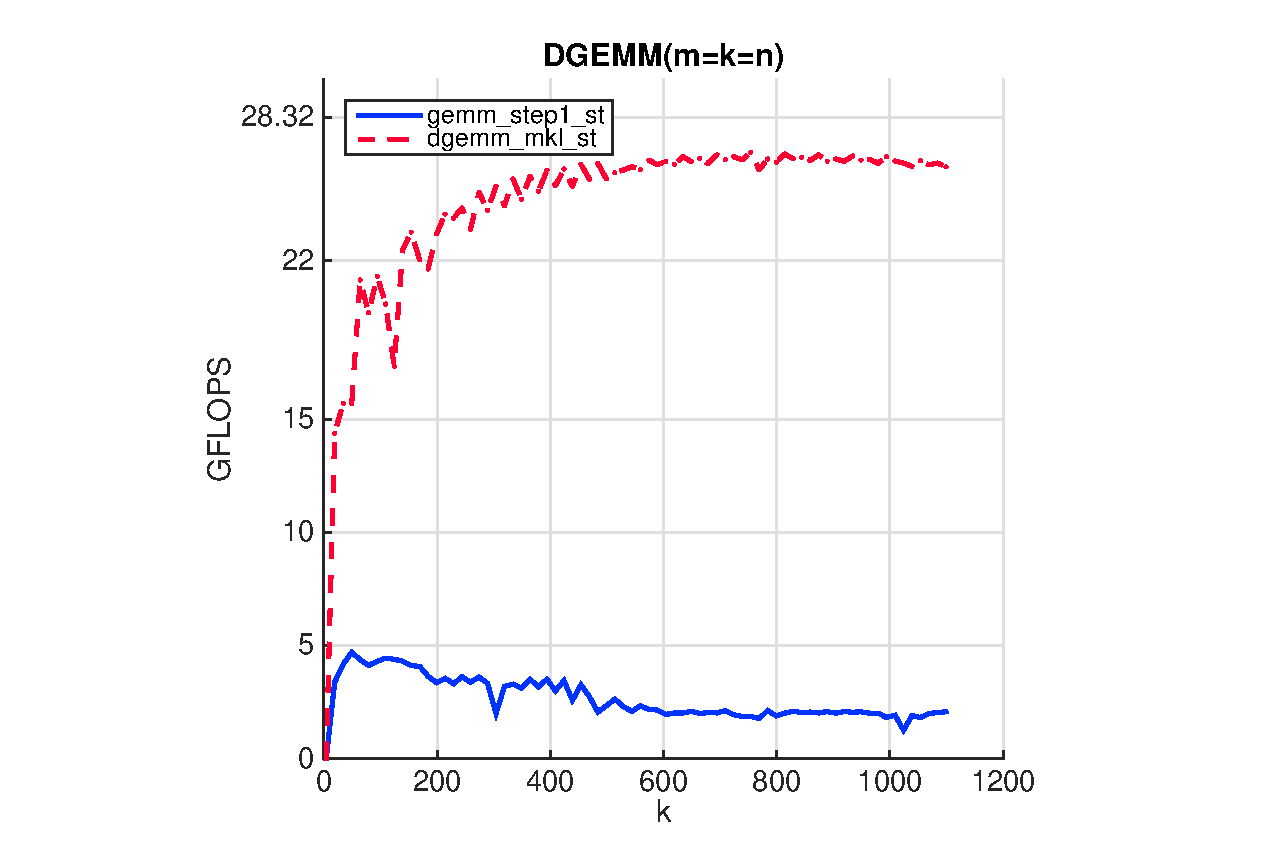
\includegraphics[scale=.5]{figures/step1_single_thread_ivy.eps}
  \caption{Step1 performance}
  \label{fig:naive}
\end{figure} 

\begin{figure}[!htp]
  \centering
  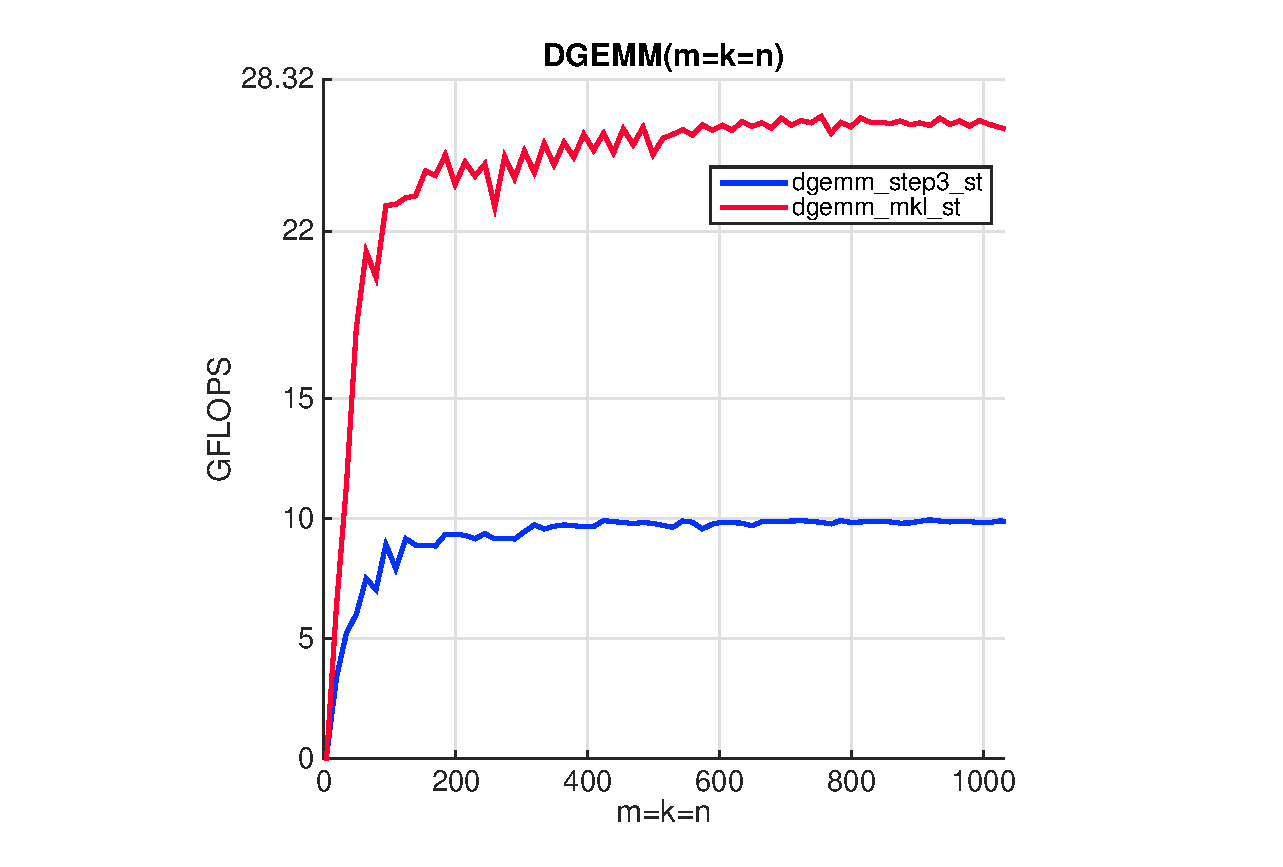
\includegraphics[scale=.5]{figures/step3_single_thread_ivy.eps}
  \caption{Step3 performance}
  \label{fig:packing}
\end{figure} 

\begin{figure}[!htp]
  \centering
  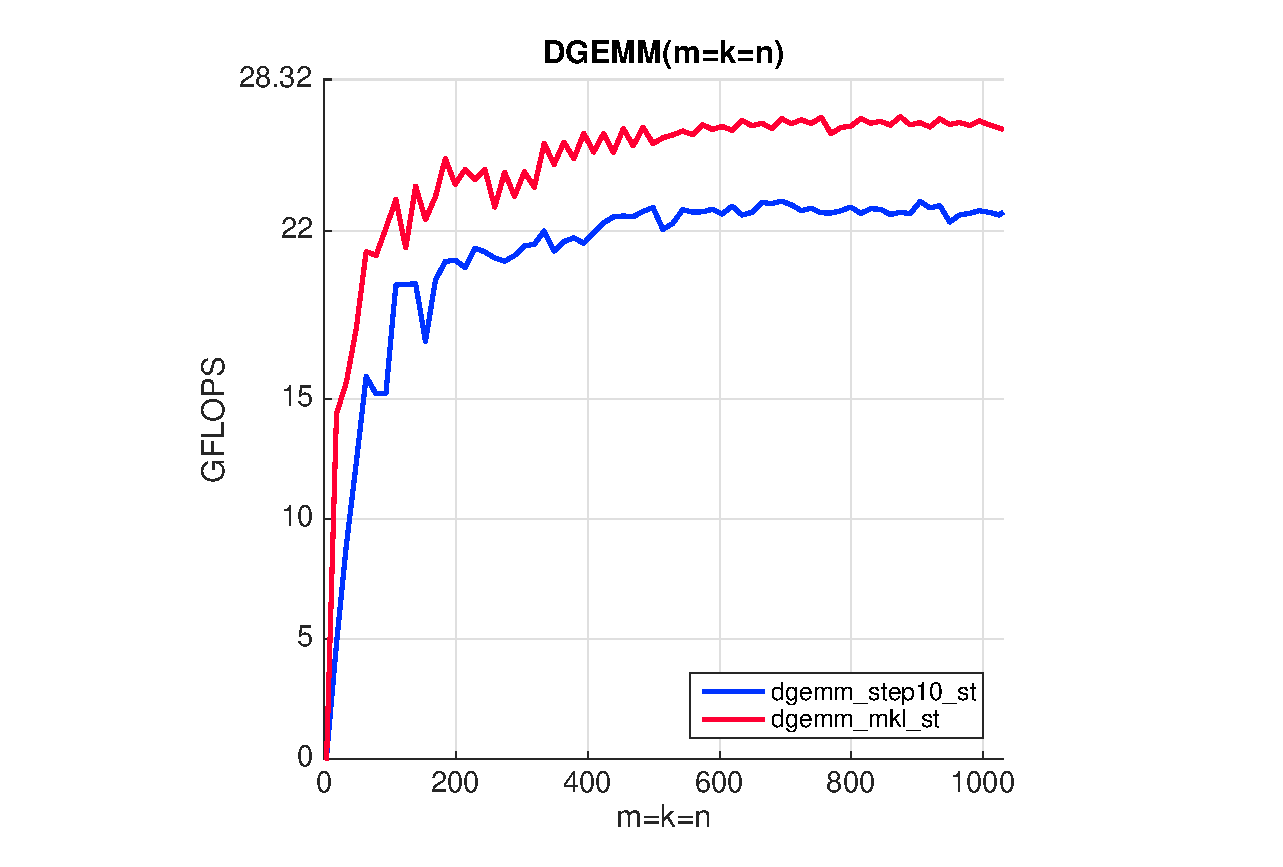
\includegraphics[scale=.5]{figures/step10_single_thread_ivy.eps}
  \caption{Step10 performance}
  \label{fig:int}
\end{figure} 

\begin{figure}[!htp]
  \centering
  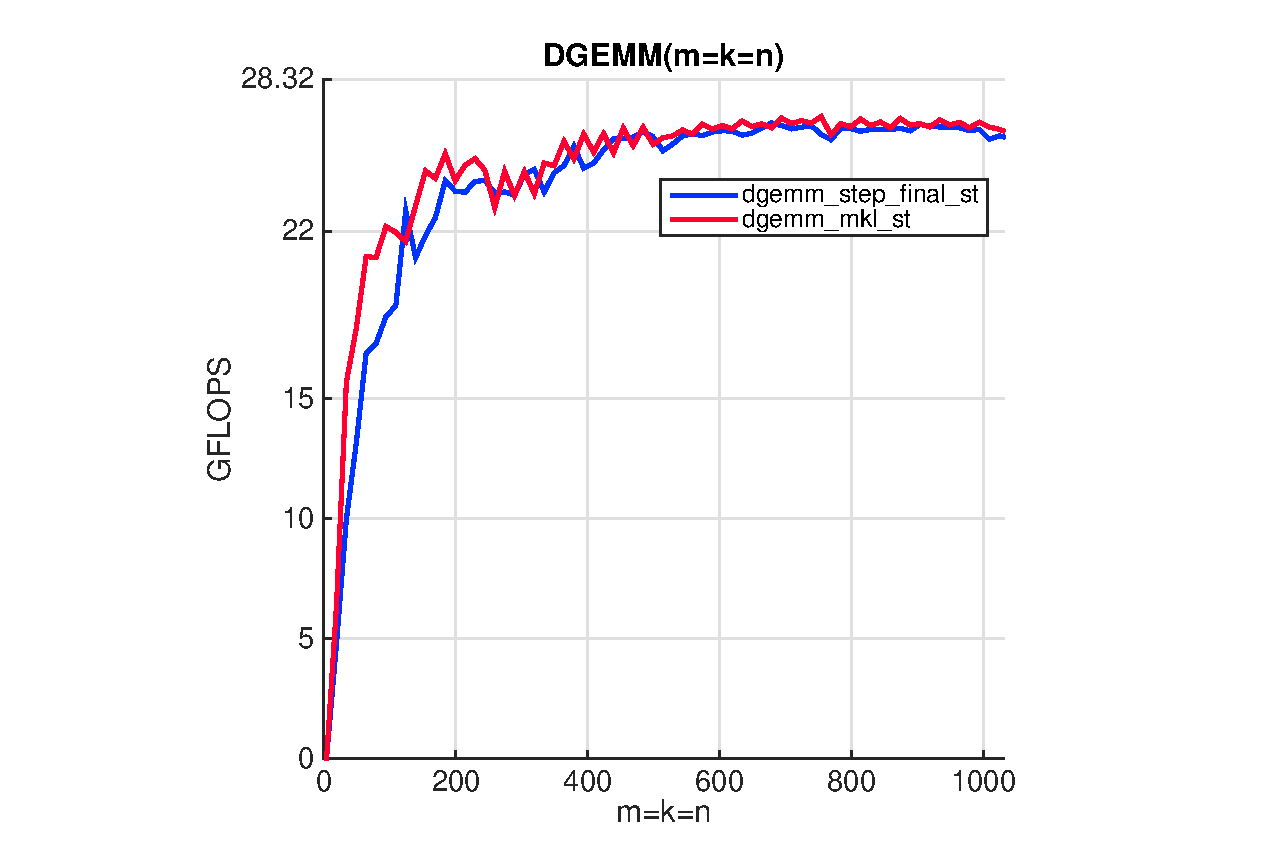
\includegraphics[scale=.5]{figures/step_final_single_thread_ivy.eps}
  \caption{Step Final performance}
  \label{fig:final}
\end{figure} 

\begin{figure}[!htp]
  \centering
  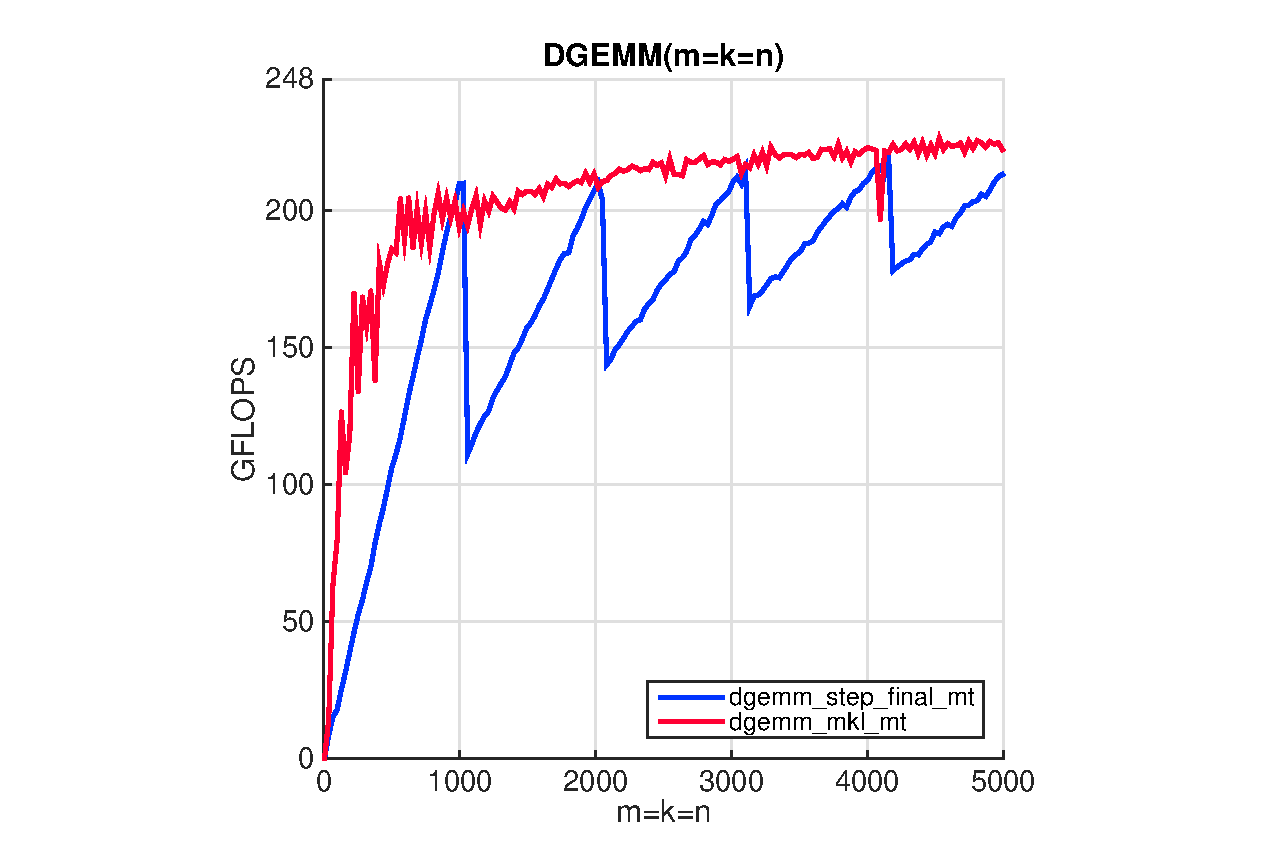
\includegraphics[scale=.5]{figures/step_final_multi_thread_ivy.eps}
  \caption{Step Final performance (multi-thread)}
  \label{fig:final_mt}
\end{figure} 







